\section{Schaltung}
\label{sec:Schaltung}

%Schaltung zeigen
%Funktionsweise der Schaltung
%Welche Tests sinnvoll und warum

In der Bachelor-Thesis von Simon Hasler ist eine Teilschaltung implementiert, welche den Strom eines Asynchronmotors misst. Diese Schaltung wurde von den Autoren ausgewählt, um im Modul EMV Tests durchführen zu können. Damit die Schaltung bei den Tests sicher nicht kaputt geht, sollte diese nachgebaut werden. Leider wurde bekannt, dass diese Teilschaltung, generiert von einer anderen, externen Schule, nicht funktionstüchtig ist. Aus diesem Grund haben die Autoren eine eigene Schaltung zur Strommessung mit an der Fachhochschule zur Verfügung stehenden Mitteln zusammengestellt. Bei der Schaltung handelt es sich um eine Strommessung über einen Widerstand (Shunt) mit Tiefpassfilterung und einem Operationsverstärker, zu sehen in Abbildung \ref{fig:SchaltungDraw}.\\

\begin{minipage}[b][6cm][t]{1\textwidth}
\centering
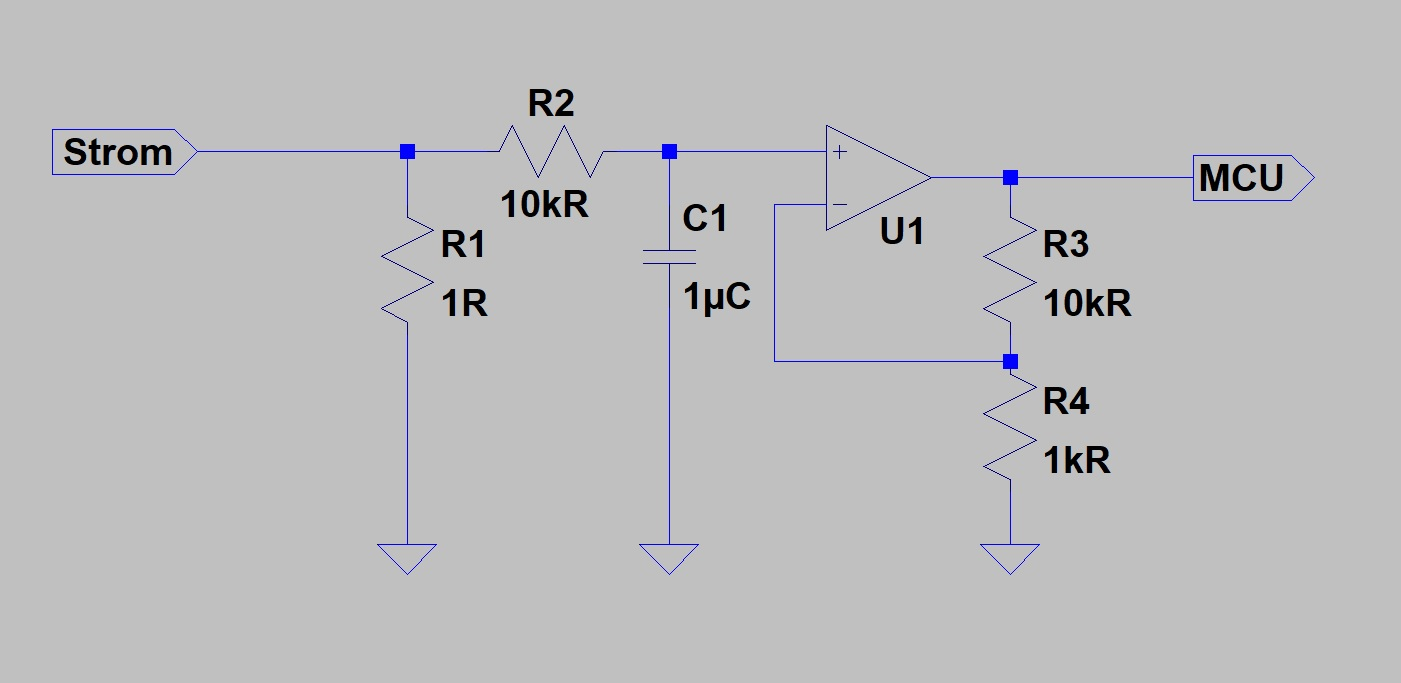
\includegraphics[angle=0,width=0.75\textwidth]{graphics/SchaltungDraw.jpg}
\captionof{figure}{Schema der entworfenen Schaltung.}
\label{fig:SchaltungDraw}
\end{minipage}
\vspace*{0.25cm}

In Abbildung \ref{fig:SchaltungDraw} ist zu sehen, dass von Links der zu messende Strom in die Schaltung hinein und durch den Shunt (R1) strömt. Ein Tiefpassfilter (R2 parallel zu C1) schützt die nachfolgende Schaltung vor Schäden durch hohe Frequenzen. Der Operationsverstärker (U1) dient als nichtinvertierender Verstärker mit einem Verstärkungsfaktor von $1+\dfrac{R3}{R4}$. Die Ausgangsspannung, welche im Verhältnis zum zu messenden Strom ist, wird an einen Mikrocontroller zur Datenverarbeitung weiteregeben (bzw. erst auf einen ADC). Der Operationsverstärker benötigt zudem eine Spannungsversorgung von +5V.\\

Das Schema wird umgesetzt mit Bauteilen, welche direkt an der Fachhochschule bezogen werden können. Ebenfalls wird nicht extra ein Print hergestellt, sondern eine Lochrasterplatine verwendet, auf welcher die Schaltung gelötet wird. Die Schaltung sieht umgesetzt aus wie in Abbildung \ref{fig:Schaltung1} aus.

\begin{minipage}[b][6cm][t]{1\textwidth}
\centering
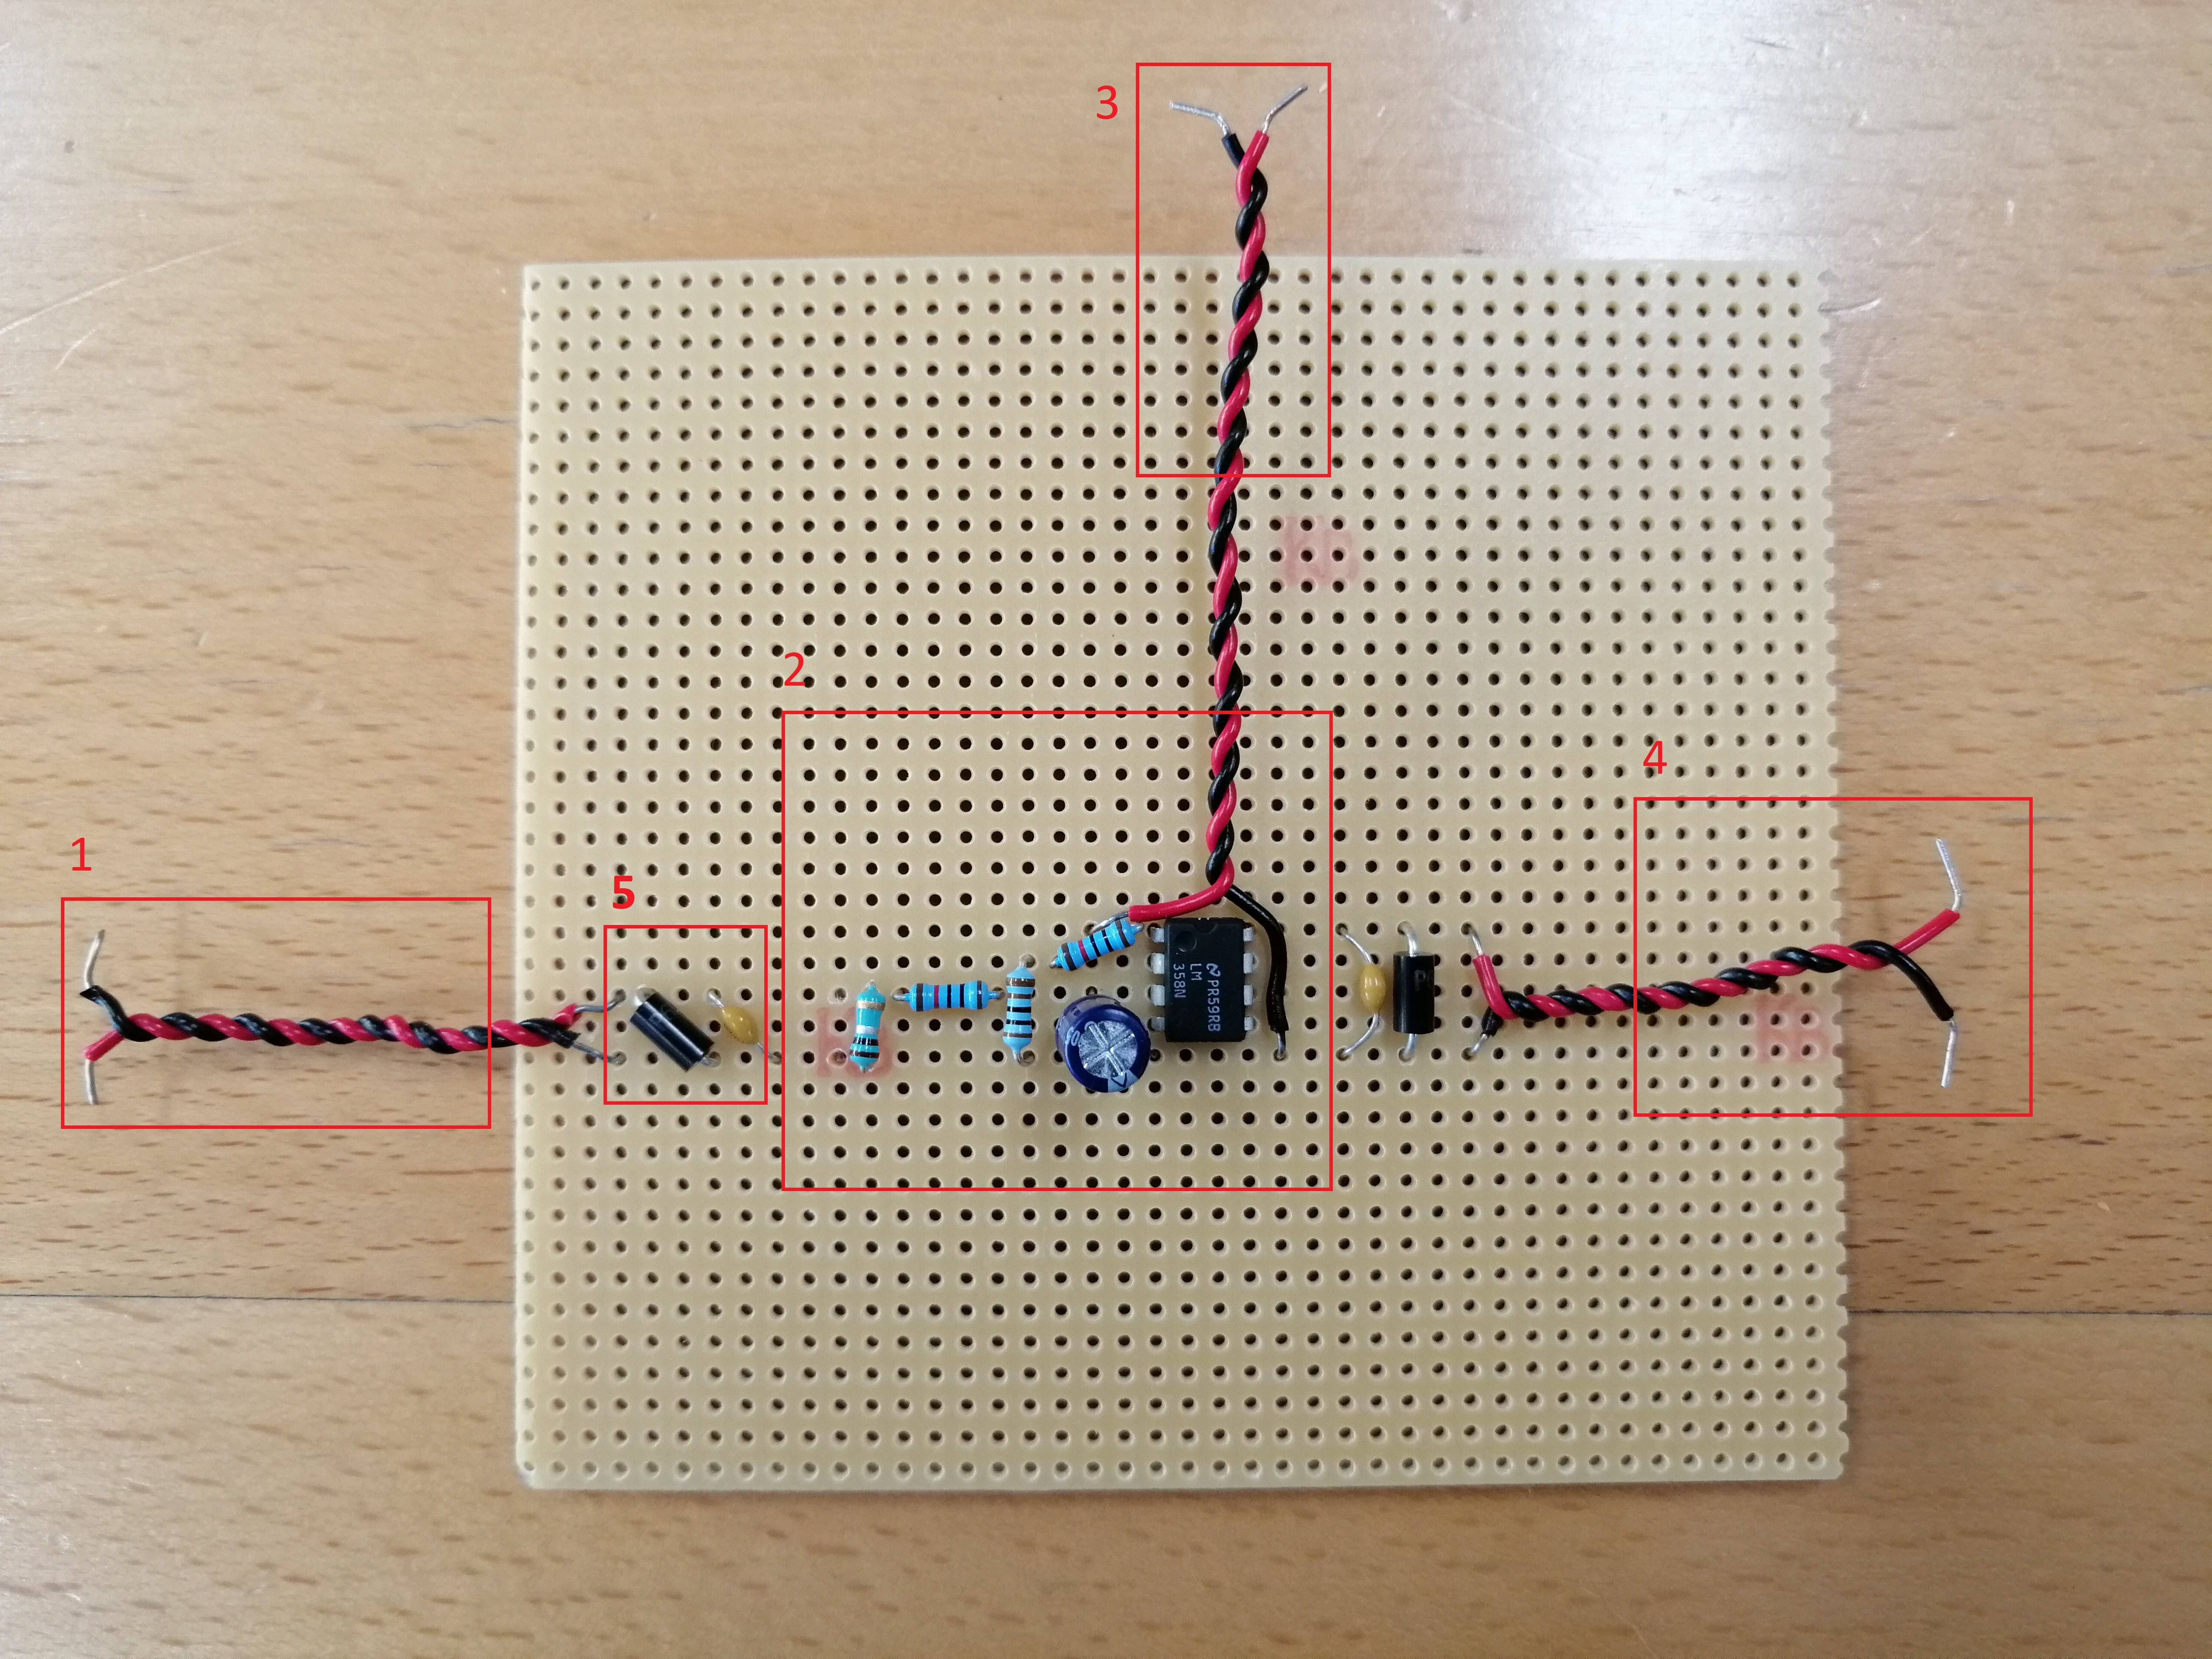
\includegraphics[angle=0,width=0.75\textwidth]{graphics/Schaltung1.jpg}
\captionof{figure}{Die realisierte entworfene Schaltung.}
\label{fig:Schaltung1}
\end{minipage}
\vspace*{4cm}

In Abbildung \ref{fig:Schaltung1} sind die Anschlüsse für eine Stromquelle (1), für den Ausgang zur MCU bzw. zum Oszilloskop (3) und für die Speisespannung des Operationsverstärkers (2) zu sehen. Die Schaltung selbst, wie in Abbildung \ref{fig:SchaltungDraw} gezeichnet, ist ebenfalls zu sehen (4). Ausserdem sind die Schutzelemente gegen die ausgewählten EMV-Störungen hier schon implementiert (5), was jedoch erst in Kapitel \ref{sec:Schutz} näher besprochen wird.\\

Damit sichergestellt ist, dass die Schaltung ihre Aufgabe erfüllt, muss dies getestet werden. Dafür wird der Ausgang an ein Oszilloskop angeschlossen, der Operationsverstärker mit einer Spannungsquelle gespiesen (5V) und am Eingang eine Stromquelle angeschlossen. Nun sollen für verschiedene Ströme auch verschiedene Spannungslevel auftreten. Die Auswertung ist zu sehen in Abbildung \ref{fig:Schaltungstest}.\\

\begin{minipage}[b][6cm][t]{1\textwidth}
\centering
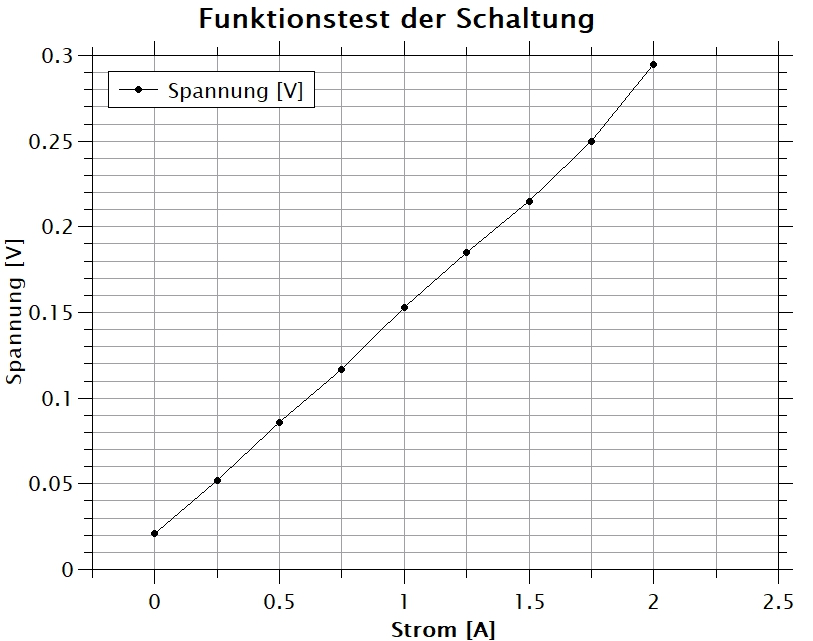
\includegraphics[angle=0,width=0.75\textwidth]{graphics/Schaltungstest.jpg}
\captionof{figure}{Die realisierte entworfene Schaltung.}
\label{fig:Schaltungstest}
\end{minipage}
\vspace*{4cm}

Abbildung \ref{fig:Schaltungstest} zeigt die am Oszilloskop gemessene Spannung für verschiedene Eingangsströme. Es fällt ein linearer Zusammenhang auf, wobei es zu kleineren Abweichung (Messfehler, Ablesefehler...) kommt. Die Schaltung gibt also für jeden Eingangsstrom einen anderen Spannungspegel aus, weshalb gesagt werden kann, dass die Schaltung funktioniert.\\

Die Schaltung wurde aufgebaut und auf ihre Funktionalität getestet. Als nächstes folgen die ausgewählten EMV-Testarten und deren Normen, auf diese hin die Schaltung getestet wird.\\


